\documentclass[12pt,letterpaper]{article}

\usepackage{amsmath, amsthm}
\usepackage{microtype, parskip}
\usepackage[comma,numbers,sort&compress]{natbib}
\usepackage{lineno}
\usepackage{docmute}
\usepackage{caption, subcaption, multirow, morefloats, rotating}
\usepackage{wrapfig}

\frenchspacing

\begin{document}

\section*{Introduction}

% regional species pool
How do species pools change over time as species are recruited or go extinct? When are ecotypes enriched or depleted? How does global and regional environmental context affect the distribution of species ecotypes (e.g. guilds) in a regional species pool?

A regional species pool is the set of species which form communities in a specific region; local communities are subsets of the regional pool. The composition of a regional species pool changes over time due to speciation, migration, extinction. Local scale processes like resource competition only affect the regional species pool if all communities are affected.

% guilds and ecocube and ecotypes
Valentine and Bambach how they presented guilds in paleobiology which is taxa united by similarity of their macroecology \citep{Valentine1969,Bambach1977}. Bush and Bambach presented an ecocube to describe what how marine invertebrates partition space and resources \citep{Bush2007,Bambach2007,Bush2011}. Unique combinations represent what possible ecotypes are observable. The distribution of ecocube occupancy is then normally analyzed as raw counts of unique combinations or using ordination methods and the change in disparity over time is estimated \citep{Bush2007,Bambach2007,Bush2011}.


% how we think about mammal diversity
Analysis of mammal diversity and hypotheses as to the processes that have shaped it tend to fall under a few categories: diversity of the whole system \citep{Alroy2000g,Alroy1996a,Figueirido2012,Liow2008}, guild based \citep{Janis2004,Janis2000,Jernvall2004,Janis1993c,Pires2015a,Janis2008a}, clade based \citep{Quental2013,Slater2015c,Silvestro2015b}, climate based \citep{Blois2009,Janis1993c,Janis1993b}, and location based \citep{Eronen2015,Badgley2013}. Rarely are more than two of these categories considered simultaneously, and instead integration of these diverse observations and hypotheses tends to be based on coincidence. The goal of this study is to pool information from multiple levels of organization by integrating both species and climate data into a single analysis in order to provide a more holistic intepretation of the processes which may have shaped mammal species diversity.


% 4th corner as similar but different lens
Fourth-corner modeling is an approach to explaining the patterns of either species abundance or presence/absence as a product of species traits, environmental factors, and the interaction between traits and environment \citep{Brown2014c,Warton2015a,Pollock2012,Jamil2013} CITATION. In modern ecological studies, what is being modeled is species occurrences at localities distributed across a region \citep{Pollock2012,Jamil2013}. In this study, what is being modeled is the pattern of species occurrence over time for most of the Cenozoic in North America (Fig. \ref{fig:concept_fourth_corner}). These two approaches, modern and palentologicial, are different views of the same three-dimensional pattern: species at localities over time. The temporal limitations of modern ecological studies and difficulties with uneven spatial occurrences of fossils in paleontological studies means that these approaches are complimentary but reveal different patterns of how species are distributed in time and space.

\begin{figure}[ht]
  \centering
  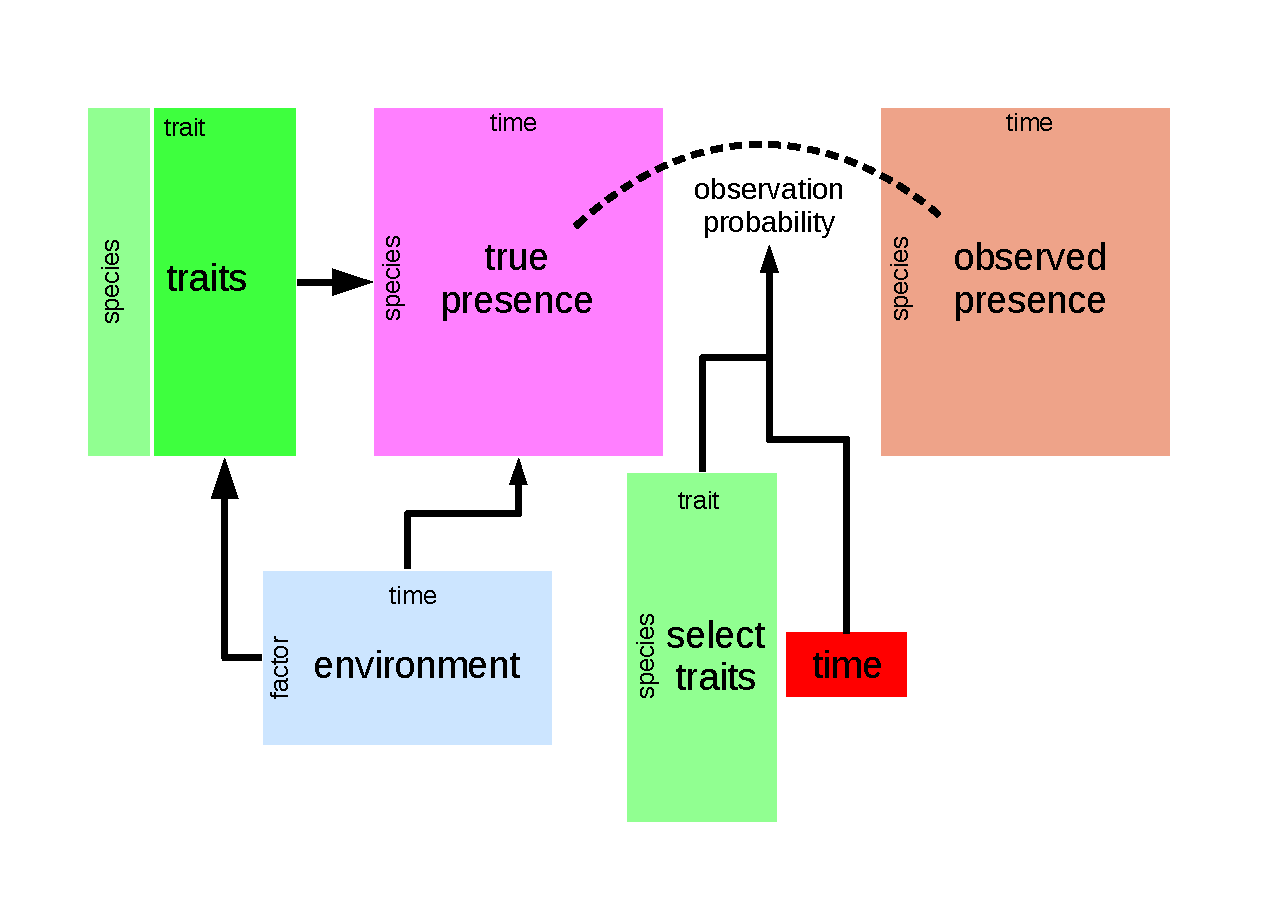
\includegraphics[width=\textwidth,height=0.8\textheight,keepaspectratio=true]{figure/paleo_fourth_corner}
  \caption[Conceptual diagram of the paleontological fourth-courner problem]{Conceptual diagram of the paleontological fourth corner problem. The observed presence matrix (orange) is the empirical presence/absence pattern for all species for all time points; this matrix is an incomplete observation of the ``true'' presence/absence pattern (purple). The estimated true presence matrix is modeled as a function of both environmental factors over time (blue) and multiple species traits (green). Additionally, the affect of environmental factors on species traits are also modeled as traits are expected to mediate the effects of a species environmental context. This diagram is based partially on material presented in \citet{Brown2014c} and \citet{Warton2015a}.}
  \label{fig:concept_fourth_corner}
\end{figure}

One of the greatest challenges with analyzing species occurrence data is the inherent incompleteness of any sample \citep{Royle2008,Royle2014,Foote1999a,Foote2001,Lloyd2011,Wang2016b}. In the modern, only presences are certain as an absence can be caused by both the species being truly absent or the species never having been sampled \citep{Royle2008,Royle2014}. For paleontological data in the context of this study, the incomplete preservation of fossil communities combined with the incomplete sampling of what fossils there are means that the true times of origination or extinction may not be observed \citep{Foote1999a,Foote2001,Wang2015,Wang2016b}.



% what we're dealing with in terms of hypotheses
In the analyses done here, a few key covariates which describe species' macroecology and environmental context are considered. Because of the complexity of fourth-corner analyses in terms of both number of covariates considered and structure of each model, it is possible to consider and test a large number of possible hypotheses. Presented here are the species traits and related hypotheses, followed by the environmental factors and related hypotheses.

The principle species trait considered in this study is a species' ecotype, defined here as the unique combination of species dietary cateogry and locomotor category (e.g. arboreal omnivore versus unguligrade herbivore). This classification is analogous to the marine invertebrate ecocube discussed above \citep{Bush2007,Bambach2008,Bush2011}. Species mass was also included as a species trait, but is mostly included in order to control for that effect on species observation and occurrence.


% hypotheses about the effect of ecotypes
Translating previous work into hypotheses applicable to this analysis is difficult. Taxonomic grouping is frequently invoked in many proposed hypotheses for how mammal diversity is structured \citep{Quental2013,Slater2015c,Janis1993c,Pires2015a,Janis2008a}. However, this practice is problematic because taxonomic grouping conflates shared evolutionary history and similarities in species macroecology which means that whatever aspects of species biology are important for the processes underlying species diversity are obscured.

\citet{Jernvall2004} found that for the Neogene of Europe the relative abundance of mammal guilds was stable over time even in the face of high turnover rates.

Many discussions of the effects or associates of species ecology and diversity have focused on ungulate herbivores \citep{Janis2004,Janis2000,Janis1993c,Janis2008a} and carnivores \citep{Pires2015a,Slater2015c,Janis1993c,Silvestro2015b}.

The diversity history of ungulate herbivores is characterized by younger originating taxa having longer legs, higher crowned teeth, and a preference for grazing over browsing than their earlier originating counterparts \citep{Janis2004,Janis2000,Janis1993c,Janis2008a}; all of which have all been attributed to environmental change or tectonic activity driving climate and environmental change \citep{Janis2008a,Eronen2015,Blois2009}. Additionally, it has been observed that ungulate cursorial forms arose before carnivore cursorial forms, an observation attributed to the reorganization of plant communities towards the end of the Cenozoic \citep{Janis1993c}.

Within the canid guild of North America (e.g. plantigrade and digitigrade carnivores) there is evidence that their diversity, or at least the structure of that diversity, is self-regulating in the sense that species from different clades are ``competing'' for niche or guild space in the North American regional species pool \citep{Silvestro2015b}.

A pattern of generally constant diversity through time is also observed within the canid carnivore subguilds of hypercarnivore, hypocarnivore, and mesocarnivores though there was no evidence of diversity-dependence in trait (e.g. body size) evolution \citep{Slater2015c}. The general pattern of constant diveristy in the face of turnover is however consistent with a possibly self-regulating system.

There is some uncertainty as to the effect of species body size on mammal diversity and aspects of the diversification processes, specifically extinction \citep{Liow2008,Liow2009,Tomiya2013,Smits2015b}.

%   difficult to tease out because people use taxonomic grouping, which conflates common ancestry and ecology
% things people have remarked upon in the past
%   cursorial carnivores are a late occurrence (Janis and Wilhelm 93 JME)
%   ungulate legs get longer over Cenozoic but due to climate change (Janis 08)
%   guilds stable in face of turnover EUROPE (jernvall and fortelius 04 amnat)
%   larger body size, greater extinction rate (liow et al 08 pnas)
%   ungulate extinction/turnover at end of eocene (janis 97)
%   browse to graze within herbivores
\citet{Smits2015b} found several systematic differences in mammal species durations associated with various species traits. Omnivorous taxa were found to have, on average, a greater duration than other dietary categories. Additionally, arboreal taxa were found to have a shorter duration than other locomotor categories. 

An unresolved question from \citet{Smits2015b} is whether the greater extinction risk faced by arboreal is constant over time or if there was a change in extinction risk at the Paleogene/Neogene boundary. Specifically, the question is whether the extinction risk arboreal taxa increased in the Neogene, driving the loss of arboreal taxa and average extinction risk of arboreal taxa down. 

There are no observed massive cross-taxonomic turnover events in the North American record, unlike the Neogene record Europe \citep{Alroy2009,Alroy1996a,Eronen2015,Janis1993b,Alroy2000g}.
% if we control for one ecotype axis, what is variation along other axis?
% digitigrade vs unguligrade herbivores
% plantigrade vs digitigrade carnivores
% modernization of ecologies?
%   this is normally talked about in terms of taxonomic groups
%   how does this translate into ecologies?




% effect of climate on diversification process
Fundamentally, all species respond differently to climate and environmental change \citep{Blois2009}. Macroecological patterns are the similarities across species, the emergent properties of how species react to a similar ``stimulus.''

The Cenozoic is generally characterized by a global cooling trend and the development of polar ice-caps during the Neogene, with a few notable exceptions \citep{Zachos2001,Zachos2008,Cramer2011}. The Cenozoic of North America is additionally characterized by an environmental transition from the closed, partially forested environments of the Paleogene to the savannah and grasslands environments of the Neogene \citep{Blois2009,Janis1993b,Janis2000,Stromberg2005}.

With respect to North America specifically, much of regional climatic and environmental change has been attributed to tectonic activity and uplift \citep{Blois2009,Eronen2015,Janis2008a,Badgley2013} CITATIONS. Additionally, tectonic activity and uplift is considered the driving causal mechanism behind both changes to diversity and trait evolution \citep{Blois2009,Badgley2013} CITATIONS.

The Eocene-Oligocene transition is associated with high extinction amongst ungulate taxa \citep{Janis2008a}. This period is also the transition from the Paleogene to the Neogene and from herbivores being browsing dominated to grazing dominated CITATION.

There is an observed stability in estimates of global temperature from the E/O transition till the end of the Miocene; this is called the Mid-Miocene climatic optimum \citep{Zachos2001,Zachos2008}. The Mid-Miocene climatic optimum is bookended by periods of temperature decline.

The environmental factors included in this study include estimates of global tempreature and the changing floral groups present in North America across the Cenozoic. These covariates were chosen because they provide high level characterizations of the environmental context of the entire North American regional species pool for most of the Cenozoic. Importantly, the effects of a species ecotype on diversity are themselves modeled as functions of environmental factors (Fig. \ref{fig:concept_fourth_corner}) allowing for inference as to how species ecology mediates environmental context. 

The effect of climate on diversity and the diversification process has been the focus of considerable research with many analyses favoring diversification being more biologically-mediated than climate-mediated \citep{Alroy1996a,Alroy2000g,Figueirido2012,Clyde1998a}. Scale of analysis makes a big difference in interpretation of results, both temporal and geographic. For example when the mammal fossil record analyzed at small temporal and geographic scales a correlation between diversity and climate are observable \citep{Clyde1998a}. However, when the record is analyzed at the scale of the continent and the Cenozoic there is no correlation with diversity and climate \citep{Alroy2000g}. This results, however, does not go against the idea that there may be short periods of correlation and that this correlation change or reverse direction over time; instead this result means that there is no single direction of correlation between diversity and climate \citep{Figueirido2012}. 

In the case of a fluctuating correlation between diversity and climate it is hard to make the argument of an actual causal link between the two without understanding the ecological differences in mammalian fauna over time; when this analysis is based on diversity or taxonomy alone no mechanisms are possible to infer. After all, taxonomy conflates many potential factors that could affect diversification into a single variable; by separating the effects of shared common ancestry (i.e. phylogeny) from species ecology the subtle differences in the diversification process can be observed \citep{Smits2015b}.




% what have people said before
%   ungulates get hit at end of Eocene b/c cool (Janis 97)
%   climate is not correlated with mammal diversity or body size (Alroy et al 2000)
%   it is all mountain building (Badgley and Finarelli 13, Eronen et al 15 ProcB, Janis 93)
%     tectonic events drive climate, climate then affects species
%     taxonomic dependence






Ultimately, the goal of this analysis are to understand when are unique ecotypes enriched or depleted in the North American mammal regional species pool and how changes in ecotypic diversity are related to changes in species' environmental context.


\end{document}
